%=========================================
% 	   Einleitung     					 =
%=========================================
\chapter{Einleitung}
%:::::::::::::::::::::::::::::::::::::::::::::::::::::::::::::::::::::::::::::::::::::::::::::::::::::::::::
\section{Motivation}
Gemäß dem Metcalfe'schen Gesetz\footnote{Das \textit{Metcalfe'sche Gesetz} (Robert Metcalfe, 1980) besagt, dass der Nutzen eines Netzwerks proportional zu der Anzahl der Verbindungen innerhalb des Netzwerkes wächst, während die Kosten proportional zu der Anzahl der Teilnehmer wachsen.} haben sich \textit{Social Media} zu einer der wichtigsten Informationsquellen unserer Zeit etabliert. Nutzer agieren nicht nur als Konsumenten, sondern immer mehr als Produzenten von Information. Unterstützt durch die Allgegenwärtigkeit des Internets, gelangen auf diese Weise exorbitante Mengen unstrukturierter Information in Echtzeit an die Teilnehmer des Netzwerks. Eine Selektion dieser Daten, etwa nach persönlichen Interessen, bleibt dem Nutzer meist selbst überlassen.
Als Inbegriff dieses Prinzips gilt der Mikroblogging-Dienst \textit{Twitter}. Nutzer des Dienstes können auf 140 Zeichen beschränkte Nachrichten - sogenannte \textit{Tweets} - verfassen und diese dann ungefiltert und ungeprüft veröffentlichen.\\\\
Ziel dieses Projektes ist es nun eine Software zu entwickeln, mit der die Selektion von Tweets automatisiert erfolgen kann. Grundlage dafür bietet die von Twitter bereitgestellte Streaming API, welche eine permanente Versorgung mit neuen Tweets sicherstellt. Diese sollen im weiteren Verlauf so strukturiert werden, dass eine individuelle Aufbereitung der Tweets ermöglicht wird. Im Vordergrund steht hierbei eine objektive Einschätzung der Tweets anhand subjektiv festgelegter Merkmale.\\\\
Die systematische Verarbeitung großer Datenmengen, im Allgemeinen unter dem Begriff \textit{Data-Mining} bekannt, stellt dabei die zentrale Herausforderung dar. Aus dem vorhandenen Datenpool soll jene, für den Nutzer relevante Information extrahiert werden, sodass individuelles Wissen generiert werden kann. Da ständig neue Daten ankommen, muss dieser Prozess ereignisgesteuert erfolgen. Um den Datenüberschuss möglichst gering zu halten, sind schnelle Entscheidungen essentiell. \\\\
In den folgenden Abschnitten werden zunächst die technischen Rahmenbedingungen im Hinblick auf die Funktionsweise der Twitter API erläutert. Es folgt eine Konkretisierung der Anforderungen in Form einer Produktvision. Anschließend wird das Projekt erst aus organisatorischer, dann aus technischer Sicht beschrieben bevor die Implementierung der einzelnen Teilbereiche detailliert betrachtet wird. Im Rahmen einer Evaluation sollen abschließend einige Qualitätsmerkmale bezüglich Organisation und Umsetzung des Projektes untersucht werden.
\newpage
%:::::::::::::::::::::::::::::::::::::::::::::::::::::::::::::::::::::::::::::::::::::::::::::::::::::::::::
\section{TwitterStream API}
%
Die \textit{Twitter Streaming APIs} bieten eine öffentlich zugängliche Programmierschnittstelle für einen Echtzeit-Zugriff auf Daten der Social Mediaplattform \textit{Twitter} auf der Grundlage von HTTP. Eine Webanwendung, die ihrem Endnutzer Daten eines Dritten zur Verfügung stellt, arbeitet stets einerseits als Server für die Clientanwendung des Nutzers und ist andererseits selbst Client eines Datenservers, in diesem Fall Twitter. Der hergebrachte Weg zu online verfügbaren Daten, sowohl für Twitter als auch bei anderen Diensten wie \textit{Facebook} oder \textit{GoogleEarth}, erfolgt über eine REST API. Dabei stellt eine auf REST basierende Webanwendung, meist auf Anfrage eines Benutzers mittels eines HTTP-Requests, mit dem bestimmte Suchparameter übermittelt werden, eine entsprechende Anfrage beim Server des Anbieters der Daten. Er erhält die gewünschten Daten in der Response und gibt sie an den Benutzer weiter. Die Anfrage vollzieht sich dabei zustandslos. Für jede Anfrage wird eine neue \acs{TCP}-Verbindung zum Anbieter aufgebaut, die wie jede HTTP-Verbindung nach der Übermittlung der Daten sofort wieder durch den Anbieter-Server beendet wird.
%
\begin{figure}[!h]
    \centering
    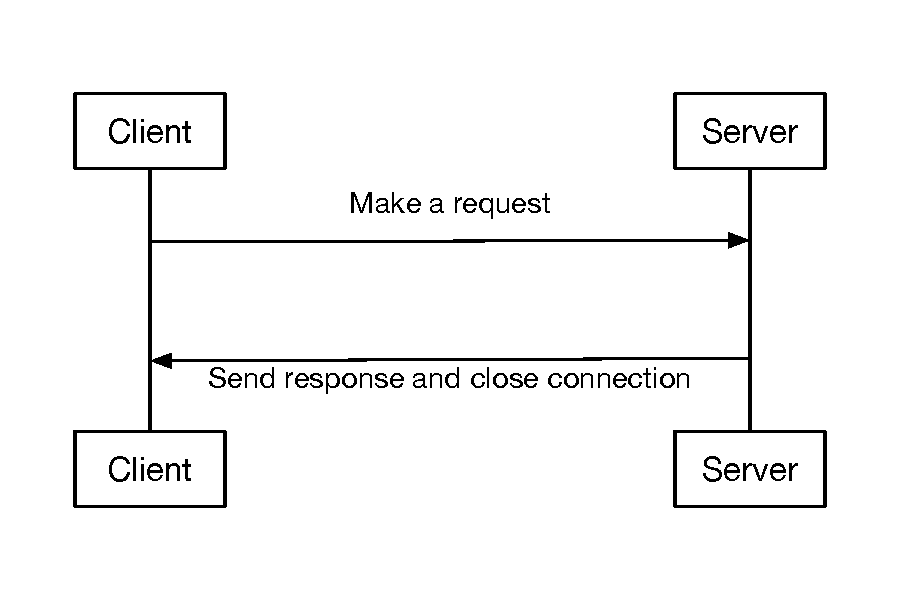
\includegraphics[width=0.85\textwidth]{Graphics/normal_rest_api}
    \caption[Grundprinzip einer REST-API, in Anlehnung an \cite{quora:api}]{Grundprinzip einer REST-API \cite{quora:api}}
   \label{fig:restapi}
\end{figure}
%
Das Prinzip einer Streaming API beruht dagegen gerade darauf, die Verbindung zum Datenserver über einen längeren Zeitraum aufrecht zu erhalten. Die Verbindung wird auch hier durch einen Request eingeleitet, in dem gewisse Such- oder vielmehr Filterparameter enthalten sind. Doch der Datenserver antwortet nicht unverzüglich mit bestimmten vorliegenden Daten und beendet die Verbindung, sondern hält die Verbindung aufrecht und sendet Informationen über zu den Suchparametern passende Ereignisse in Echtzeit. Auf der Client-Seite, also in der Webanwendung, können diese Informationen dann aus dem Socket der Verbindung gelesen werden.
%
\begin{figure}[!h]
    \centering
    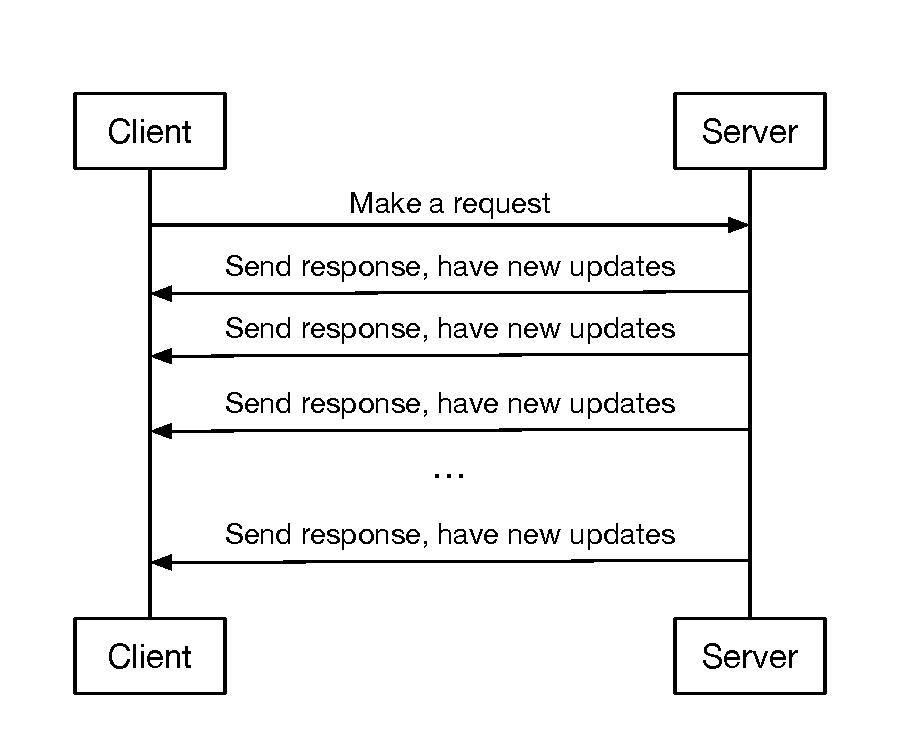
\includegraphics[width=0.85\textwidth]{Graphics/streaming_api}
    \caption[Grundprinzip einer Streaming-API, in Anlehnung an \cite{quora:api}]{Grundprinzip einer Streaming-API \cite{quora:api}}
   \label{fig:streamapi}
\end{figure}
%
Dieser Unterschied führt auch zu einer anderen allgemeinen Architektur eines Anwendungsservers, der eine Streaming API verwendet. Bei Verwendung einer \acs{REST} API wird eine Anfrage meist von einem Benutzer eingeleitet und vom Anwendungsserver an die Schnittstelle weitergereicht. Die erhaltenen Daten werden nicht langfristig gespeichert, sondern nach eventueller Bearbeitung direkt an den Benutzer geliefert. Eine permanente Verbindung kann hingegen nicht ständig durch den Benutzer überwacht werden und muss deshalb von der Serversoftware verwaltet werden. Die empfangenen Daten werden für den künftigen Zugriff gespeichert. Während die Serversoftware im Falle einer auf REST basierenden Anwendung also aus einer Einheit besteht, die sowohl für die Interaktion mit dem Nutzer als auch mit dem Datenserver verantwortlich ist, lassen sich bei einer typischen Streaming API zwei Teile unterscheiden. Der eigentliche Stream wird von einem abgeschlossenen Modul unabhängig vom Nutzer aufgebaut und verwaltet. Dabei handelt es sich im Grunde genommen um eine Clientanwendung zum Twitter-Datenserver. Er erhält seine Suchparameter aus einer Datenbank, in der auch die empfangenen Daten gespeichert werden. Der Zugang zu diesen Daten durch den Nutzer wird etwa durch ein Webinterface hergestellt, für das der zweite Teil der Anwendung als Server zuständig ist.
\\\\
Twitter bietet insgesamt vier Streaming-Schnittstellen an. Im Zentrum des Projekts steht der \textit{Public Stream}.\footnote{Für eine nähere Beschreibung der möglichen Parameter und ihrer Beschränkungen siehe \\ https://dev.twitter.com/streaming/reference/post/statuses/filter} Dieser wird neben anderen Suchparametern, wie Standort oder Sprache, vor allem mit einer Liste von bis zu 400 Schlüsselwörtern initialisiert. Jeder neue Tweet, der einem oder mehreren Keywords entspricht, wird durch den Stream empfangen. Das mögliche Datenvolumen ist also nur durch die Anzahl an Parametern begrenzt, während alle Tweets, die den Parametern entsprechen, erfasst werden. Allerdings ist es seitens Twitter vorgesehen, dass nur ein Public Stream pro Anwendung existiert. Daneben werden außerdem noch \textit{User Streams} und \textit{Site Streams} angeboten, die alle Tweets liefern, welche mit einem bestimmten Twitternutzer in Verbindung stehen.\footnote{\textit{Site Streams} sind die Multi-User-Version der \textit{User Streams}.} Der \textit{Firehose Stream} liefert schließlich bedingungs- und ausnahmslos alle öffentlich zugänglichen Tweets. Er ist jedoch nicht allgemein zugänglich, sondern bedarf einer Freischaltung durch Twitter.
%
\section{Produktvision}
%
Soziale Medien haben ein gespaltenes Image. Einerseits gehören sie unumstritten zum Leben im 21. Jahrhundert. Kaum ein Ereignis wird nicht durch Twitter, Facebook und andere dokumentiert und kommentiert, wenn diese Plattformen nicht sogar als Katalysator wirken, durch den ein Ereignis erst weltweit bekannt wird. Andererseits besteht bei der Teilnahme an dieser neuen Form der Kommunikation auch immer die Gefahr von ihr vereinnahmt zu werden. Jede neue Form von sozialem Medium bildet einen eigenen Mikrokosmos, dessen Regeln befolgt werden müssen, um die angebotenen Informationen nutzen zu dürfen oder zu können.\footnote{In Hinsicht auf die Einhaltung von Verhaltensregeln bzw. dem Verständnis des Jargons} Nicht zuletzt setzt man sich durch die Mitgliedschaft in einem sozialen Netzwerk immer auch zugleich einer höheren Wahrscheinlichkeit aus selbst zum Diskussionsstoff zu werden. Die Alternative zur aktiven Teilnahme an sozialen Medien, das Rezipieren einer Auswahl von Beiträgen zu einem Thema durch ein traditionelles Medium, etwa die Tagesschau, macht wiederum gerade den Vorteil einer ungefilterten Meinung im Internet zunichte. Es bedarf im Internet einer Möglichkeit für Außenstehende die Kommunikation in sozialen Netzwerken nach eigenem Ermessen zu beobachten. Durch Anwendungen nach dem REST-Prinzip sind nur gezielte Zugriffe auf die Vergangenheit möglich. Es fehlt jedoch eine Möglichkeit, um auf die aktuelle Kommunikation zugreifen zu können. \\
Das Ziel dieses Projekts ist es diese Lücke zu schließen. Es wird eine Webanwendung erstellt, in der sich Benutzer mit einem möglichst geringen Verwaltungsüberbau anmelden und beliebige Schlüsselwörter anlegen können, die ihren Interessen entsprechen. Diese werden zur Schlüsselwortliste eines Public Streams hinzugefügt, so dass sämtliche Tweets, die sie enthalten, während der Abwesenheit des Nutzers erfasst und in einer Datenbank gespeichert werden. Dem Nutzer stehen die seinen Schlüsselwörtern entsprechenden Tweets in einer Übersicht zur Verfügung, die er selbst noch einmal nach beliebigen Schlüsselwörtern und anderen Parametern filtern kann. Um den Vorteil des Echtzeitzugriffs auf aktuelle Ereignisse durch einen Stream voll auszunutzen, soll dem Benutzer außerdem die Möglichkeit gegeben werden, seine E-Mail-Adresse zu hinterlassen, so dass er automatisch über neu eingetroffene Tweets unterrichtet wird.

